\section{Overview} %%%%%%%%%%%%%%%%%%%%%%%%%%%%%%%%%%%%%%%%%%%%%%%%%%
\label{sec:over}

A \emph{heterarchy} is a partially ordered set $(H,\subtype)$ where $H$ is a set 
of classes and $\subtype$ is reflexive, transitive and anti-symmetric 
\emph{subtyping relation} on $H$. We are going to use terms \emph{class} and \emph{type}  
interchangibly as the exact distinction is not important for this discussion. 
Given two types in a subtyping relation $D \subtype B$, the type $D$ is said to be a 
\emph{subtype} or a \emph{derived class} of $B$, which in turn is said to be a 
\emph{supertype} or a \emph{base class} of $D$. When the transitive reduction 
$\subtypeD$ of $\subtype$ is a function, $H$ is usually referred to as 
\emph{hierarchy} to indicate single inheritance.

Subtyping effectively makes objects belong to multiple types. We call by the 
\emph{most-derived type} the type used to create an object (before any 
conversions). By \emph{static type} we call the type of an object as known to 
the compiler based on its declaration as well as any supertype of it. By 
\emph{dynamic type} of an object we call any base class of the most-derived type.

\subsection{Type Switch}

%This section generalizes pattern matching of closed algebraic datatype values
%to case analysis of hierarchical and extensible datatype values.
In general, \emph{type switch} or \emph{typecase} is a multiway branch statement 
that distinguishes values based on their type. In a multi-paradigm programming 
language like C++ that supports in various forms parametric, ad-hoc and 
subtyping polymorphisms, such a broad definition subsumes numerous different type 
casing constructs studied in the literature~\cite{Intensional95,Glew99,OpenShutTypecase05}. 
In this work we only look at type casing scenarios based on dynamic polymorphism 
of C++ (nominative subtyping polymorphism based on inheritance), similar to 
those studied by Glew~\cite{Glew99}. It is possible to generalize type casing 
(the notion, not our implementation) to static polymorphism of C++ (ad-hoc and 
parametric polymorphisms enabled by overloading and templates) along the line of 
work introduced by Harper and Morrisett~\cite{Intensional95} and studied in the
context of closed and extensible solutions by Vytiniotis et 
al~\cite{OpenShutTypecase05}, but we do not address such a generalization here. 
We use the term \emph{type switch} instead of a broader \emph{typecase} to 
stress the run-time nature of the type analysis similar to how regular 
\code{switch}-statement of C++ performs case analysis of values at run time.

Given an object descriptor, called \emph{subject}, of static type \code{S} 
(pointer or reference) referred to as \emph{subject type}, and a list of 
\emph{target types} \code{Ti} associated with the branches, a type switch 
statement needs to identify a suitable clause $m$ (or absence of such) based on 
the most-derived type \code{D <: S} of the subject as well as suitable 
conversion that csts the subject to the target type \code{Tm}.  
Due to multiple inheritance, types \code{Ti} in general may or may not be 
derived from \code{S}, however, because of the strong static type safety 
requirement, the type of applicable clause \code{Tm} will necessarily have to be 
one of subject's dynamic types: \code{D <: Tm}. A hypothetical type switch 
statement, not currently supported by C++, may look as following:

\begin{lstlisting}[keepspaces]
switch (subject) { case T1: s1; ... case Tn: sn; }
\end{lstlisting}

\noindent
There is no need for an explicit \emph{default clause} in our setting because 
such a clause is semantically equivalent to a case clause guarded by the 
subject type: \code{case S: s}. The only semantic difference such a choice 
makes is in the treatment of null-pointers, which, one may argue, should be 
handled by the default clause. We disagree, because not distinguishing between 
invalid object and valid object of a known static but unknown dynamic type may 
lead to some nasty run-time errors.

Similar control structures exist in many programming languages, e.g. 
\emph{match} in Scala~\cite{Scala2nd}, \emph{case} in Haskell~\cite{Haskell98Book} and 
ML~\cite{ML90}, \emph{typecase} in Modula-3~\cite{Modula3TS} and CLOS~\cite{??} (as a 
macro), \emph{tagcase} in CLU~\cite{CLURefMan}, \emph{union case} in Algol 68 
and date back to at least Simula's \emph{Inspect} statement~\cite{Simula67}. 
The statement in general can be given numerous plausible semantics:

\begin{itemize}
\setlength{\itemsep}{0pt}
\setlength{\parskip}{0pt}
\item \emph{First-fit} semantics will evaluate the first statement $s_i$ such 
      that $T_i$ is a base class of $D$
\item \emph{Best-fit} semantics will evaluate the statement corresponding to the 
      most-derived base class $T_i$ of $D$ if it is unique (subject to 
      ambiguity)
\item \emph{Exact-fit} semantics will evaluate statement $s_i$ if $T_i=D$.
\item \emph{All-fit} semantics will evaluate all statements $s_i$ whose guard 
      type $T_i$ is a subtype of $D$ (order of execution has to be defined)
\item \emph{Any-fit} semantics might choose non-deterministically one of the 
      statements enabled by all-fit
\end{itemize}

\noindent
The list is not exhaustive and depending on a language, any of these semantics 
can be a plausible choice. Functional languages, for example, often prefer 
first-fit semantics because it is similar to case analysis in mathematics. 
Object-oriented languages would typically be inclined to best-fit semantics due 
to its similarity to overload resolution and virtual dispatch, however, some 
do opt for first-fit semantics to mimic the functional style: e.g. Scala~\cite{Scala2nd}. 
Exact-fit semantics can often be seen in languages supporting discriminated 
union types: e.g. variant records in Pascal, Ada and Modula-2, oneof and variant 
objects in CLU, unions in C and C++ etc.
All-fit and any-fit semantics might be seen in languages based on predicate 
dispatching~\cite{ErnstKC98} or guarded commands~\cite{EWD:EWD472}, where a 
predicate can be seen as a characteristic function of a type, while logical 
implication can be seen as subtyping.

\subsection{Expression Problem}

Type switching is related to a more general problem manifesting the differences 
in functional and object-oriented programming styles.

%The ideas and the library were motivated by our unsatisfactory experiences 
%working with various C++ front-ends and program analysis 
%frameworks~\cite{Pivot09,Phoenix,Clang}.
%The problem was not in the frameworks per se, but in the fact that we had to use
%the \emph{visitor design pattern}~\cite{DesignPatterns1993} to inspect, traverse, and 
%elaborate abstract syntax trees to target languages. We found visitors 
%unsuitable to express our application logic directly, surprisingly hard to teach 
%students, and often slower than hand-crafted workaround techniques. Use of 
%dynamic casts in many places, often nested, to answer simple structural 
%questions, shows that the users preferred shorter, cleaner, and more direct code 
%to visitors, even at a high cost in performance (providing they understood the cost).
%
%A lot has been written about the visitor design pattern~\cite{DesignPatterns1993,Palsberg98,Zenger:2001,Oliveira08}. 
%Its advantages include \emph{extensibility of functions}, \emph{speed}, and, 
%\emph{being a library solution}. Nevertheless, the solution is \emph{intrusive}, 
%\emph{specific to hierarchy}, and requires a lot of \emph{boilerplate code} to 
%be written. It also introduces \emph{control inversion}, and, most importantly, 
%-- \emph{hinders extensibility} of classes.
%Interestingly, as bad as visitors are, they are only trying to solve a larger 
%problem in the context of object-oriented languages.

%Expression problem is a problem of supporting in a programming language modular 
%extensibility of both data and functions at the same time. Functional languages
%allow for easy addition of new functions at the expense of disallowing new data
%variants. Object-oriented languages allow for easy addition of new variants at 
%the expense of disallowing new functions. Many attempts have been made to 
%resolve this dilema in both camps, nevertheless no universally accepted solution 
%that is modular, open and efficient has been found.

%Visitor Design Pattern has became de-facto standard in dealing with expression 
%problem in many industry-strength object-oriented languages because of two 
%factors: its speed and being a library solution. It comes at the cost of 
%restricting extensibility of data, increased verbosity and being hard to teach 
%and understand, but nevertheless, remains the weapon of choice for interacting 
%with numerous object-oriented libraries and frameworks. 

Conventional algebraic datatypes, as found in most functional languages, allow 
for easy addition of new functions on existing data types. But they fall short 
in extending data types themselves (e.g. with new constructors), which requires 
modifying the source code. Object-oriented languages, on the other hand, make 
data type extension trivial through inheritance; but the addition of new 
functions operating on these classes typically requires changes to the class 
definition. This dilemma is known as the \emph{expression problem}~\cite{Cook90,exprproblem}.

Classes differ from algebraic data types in two important ways. Firstly, they
are \emph{extensible}, for new variants can be added later by inheriting from
the base class. Secondly, they are \emph{hierarchical} and thus typically 
\emph{non-disjoint} since variants can be inherited from other variants and form 
a subtyping relation between themselves~\cite{Glew99}. In contrast, variants in 
algebraic data types are \emph{disjoint} and \emph{closed}.
Some functional languages e.g. ML2000~\cite{ML2000} and its predecessor, Moby, 
were experimenting with \emph{hierarchical extensible sum types}, which are 
closer to object-oriented classes then algebraic data types are, but, 
interestingly, they provided neither traditional nor efficient facilities for 
performing case analysis on them.

Zenger and Odersky later refined the expression problem in the context of 
independently extensible solutions~\cite{fool12} as a challenge to find an 
implementation technique that satisfies the following requirements:

\begin{itemize}
\setlength{\itemsep}{0pt}
\setlength{\parskip}{0pt}
\item \emph{Extensibility in both dimensions}: It should be possible to add new 
      data variants, while adapting the existing operations accordingly. It 
      should also be possible to introduce new functions. 
\item \emph{Strong static type safety}: It should be impossible to apply a 
      function to a data variant, which it cannot handle. 
\item \emph{No modification or duplication}: Existing code should neither be 
      modified nor duplicated.
\item \emph{Separate compilation}: Neither datatype extensions nor addition of 
      new functions should require re-typechecking the original datatype or 
      existing functions. No safety checks should be deferred until link or 
      runtime.
\item \emph{Independent extensibility}: It should be possible to combine 
      independently developed extensions so that they can be used jointly.
\end{itemize}

\noindent
While these requirements were formulated for extensible data type with 
disjoint variants, object-oriented languages primarily deal with 
hierarchical data types. We thus found it important to explicitly state an 
additional requirement based on the Liskov substitution principle~\cite{Lis87}:

\begin{itemize}
\setlength{\itemsep}{0pt}
\setlength{\parskip}{0pt}
\item \emph{Substitutability}: Operations expressed on more general data variants
      should be applicable to more specific ones that are in a subtyping relation 
      with them.
\end{itemize}

%Depending on the semantics of the language's subtyping relation, 
%substitutability requirement may turn pattern matching into an expensive 
%operation. OCaml, for example, that uses structural subtyping on its object 
%types, does not offer pattern 

\noindent
We will refer to a solution that satisfies all of the above requirements as \emph{open}. 
Numerous solutions have been proposed to dealing with the expression problem in both 
functional~\cite{garrigue-98,LohHinze2006} and object-oriented 
camps~\cite{Palsberg98,Krishnamurthi98,Zenger:2001,runabout}, but very few has 
made its way into one of the mainstream languages. We refer the reader to Zenger 
and Odersky's original manuscript for a discussion of the approaches~\cite{fool12}.
Interestingly, most of the discussed object-oriented  
solutions were focusing on the visitor design pattern and its extensions, 
which even today seems to be the most commonly used approach to dealing with the 
expression problem in object-oriented languages.

A lot has been written about the visitor design pattern~\cite{DesignPatterns1993,Palsberg98,Zenger:2001,Oliveira08}. 
Its advantages include \emph{extensibility of functions}, \emph{speed}, and, 
\emph{being a library solution}. Nevertheless, the solution is \emph{intrusive}, 
\emph{specific to hierarchy}, and requires a lot of \emph{boilerplate code} to 
be written. It also introduces \emph{control inversion}, and, most importantly, 
-- \emph{hinders extensibility} of classes.

%In this work we are not trying to solve the expression problem in its full 
%generality. Instead, we concentrate on deficiencies of the visitor design 
%pattern independently of its relation to the expression problem and advocate for 
%a solution that suits object-oriented paradigm better than visitors do.

\subsection{Open Type Switch}

Note that the presence of a type switch in an object-oriented language alone 
does not solve the expression problem because the existing code may have to be 
modified to take new variants into account. Relying on default clause is not 
considered to be an acceptable solution in this context, because often times the 
only reasonable default behavior is to raise an exception. Zenger and Odersky 
note that in such cases defaults will transform type errors that should manifest 
statically into runtime exceptions that are thrown dynamically~\cite{fool12}.

While we generally agree with this observation, we would like to point out that 
in our experience newly added variants were more often extending an existing 
variant than creating an entirely disjoint one. In a hypotetical compiler, for 
example, a new kind of type expression will typically extend a 
\code{TypeExpression} variant, while a new form of annotation will extend an 
\code{Annotation} variant, thus not extending the root \code{ASTNode} directly. 
Due to substitutability requirement such a new variant will be treated as a 
variant it extends in all the existing code. The functions that will be affected 
by its addition and thus have to be modified will be limited to functions 
directly analyzing the variant it extends and not providing a default behavior.

To account for this subtlety of extensible hierarchical data types, we use a 
term \emph{open type switch} to refer to a type switch that satisfies all the 
requirements of an \emph{open solution to expression problem} stated above 
except for the \emph{no modification or duplication} requirement. We loosen it 
to allow modification of functions for which the newly added variant becomes a 
disjoint (orthogonal) case not handled by default clause. We believe that the 
loosened requirement allows us to express pragmatically interesting restrictions 
that developers are willing to live with. Besides, open type switch overcomes 
all the major shortcomings of the visitor design pattern:

\begin{itemize}
\setlength{\itemsep}{0pt}
\setlength{\parskip}{0pt}
\item Case analysis with an open type switch is \emph{non-intrusive} as it 
      inspects the hierarchy externally and can be applied retroactively. 
\item New variants can be accounted for in the newly written code and will be 
      seen as a base class or default in the existing code.
\item The affected functions are limited to those for which the newly added 
      variant is a disjoint case.
\item The code avoids the control inversion and the need for boilerplate code 
      that visitors introduce, and is thus a more direct expression of the 
      intent.
\end{itemize}

\subsection{C++ Specifics: Subobjects}
\label{sec:specifics}

C++ supports two kinds of inheritance: \emph{non-virtual}~\cite{CPPARM90} (also 
known as \emph{replicated}~\cite{RF95} or \emph{repeated}~\cite{WNST06}) 
inheritance and \emph{virtual}~\cite{CPPARM90} (or \emph{shared}~\cite{WNST06}) 
inheritance. The difference between the two only arises in situations where a 
class indirectly inherits from the same base class via more than one path in the 
hierarchy. Different kinds of inheritance give raise to the notion of 
\emph{subobject} in C++, which are then used to define semantics of operations 
like casts, virtual function dispatch etc. We give an informal introduction to 
them here in order to show some subtleties of the C++ inheritance model, which 
must be taken into account when addressing type switching or subtype testing.

\begin{figure}[htbp]
  \centering
    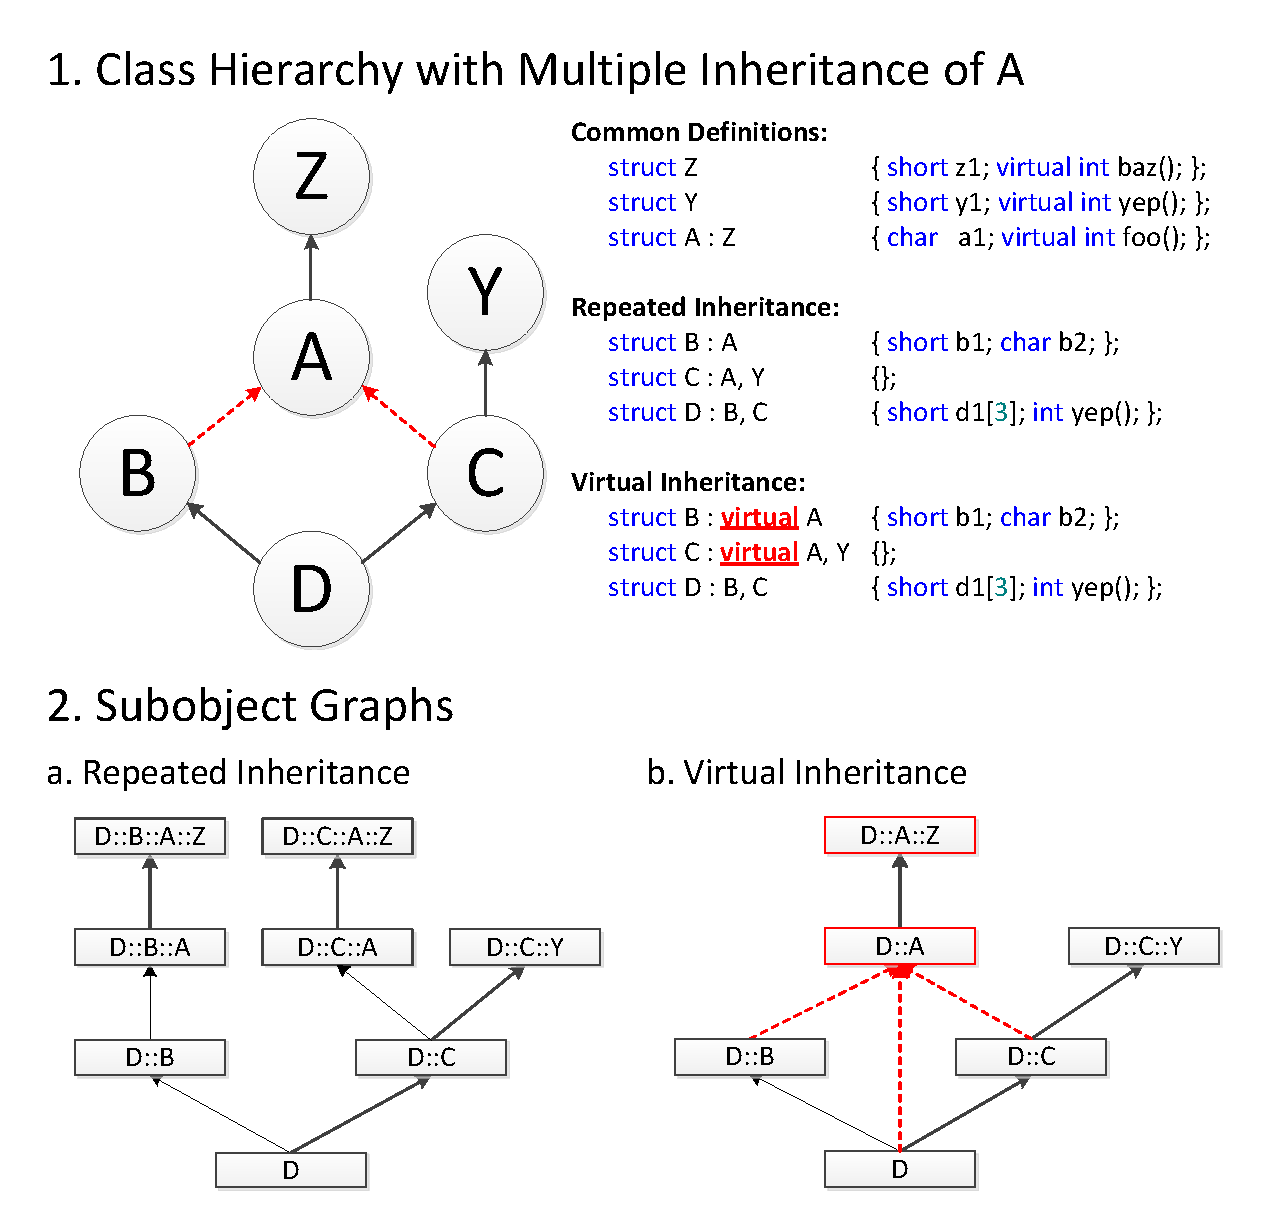
\includegraphics[width=0.47\textwidth]{Inheritance.pdf}
  \caption{Multiple Inheritance in C++}
  \label{fig:inheritance}
\end{figure}

\noindent
Consider a simple class hierarchy in Figure~\ref{fig:inheritance}(1). Class 
\code{D} indirectly inherits from class \code{A} through its \code{B} and 
\code{C} base classes. In this case, the user may opt to keep distinct 
subobjects of class \code{A} (repeated inheritance) or a shared one (virtual 
inheritance) by specifying how \code{B} and \code{C} are inherited from 
\code{A}. The kind of inheritance is thus not a property of a given class, but a 
property of an inheritance relation between derived and base class and it is 
possible to mix the two in an object of the most-derived type. 

A class hierarchy, i.e. an inheritance graph gives rise to a subobject graph, 
where a given class node may be replicated when inherited repeatedly or left 
shared when inherited virtually. The edges in such a graph represent subobject 
containtment and are marked with whether such containtment is shared or 
exclusive. Every class $C$ in the class hierarchy will have its own subobject 
graph representing the subobject of an object of the most-derived type $C$.
Figure~\ref{fig:inheritance}(2) shows subobject graph for class \code{D} 
obtained for the class hierarchy in (1) under repeated (a) and virtual (b) 
inheritance of class \code{A} by classes \code{B} and \code{C}. The shared 
containment is indicated with the dashed arrows, while exclusive with the solid 
ones.

We will use term \emph{object descriptor} to mean either pointer or reference to 
an object, which we will use interchangably when not explicitly specified. 
An object descriptor of static type $A$ referencing an object of the most-derived 
type $C$ can be understood as any \code{*::}$A$-node in the subobject graph of $C$. Rosie 
and Friedman call $A$ an \emph{effective type} of object, while the node in the 
subobject graph representing it -- its \emph{effective subobject}. 
Casts in such a model can be understood as a change from one effective subobject 
to another. We will use terms \emph{source subobject} and \emph{target 
subobject} to refer to effective subobjects before and after the cast. Their 
static types will be refered to as as \emph{source type} and \emph{target type} 
respectively. C++ distinguishes 3 kinds of casts: upcasts, downcasts and 
crosscasts.

An \emph{upcast} is a cast from a derived class to one of its bases. When the 
base class is unambiguous, such casts are implicit and require no additional 
annotations. When the base class is ambiguous, cast failure is manifested 
statically in a form of a compile-time error. This is the case for example with 
casting \code{D} to \code{A} under repeated multiple inheritance of \code{A}, 
in which case the user needs to explicitly cast the object to \code{B} or 
\code{C} first in order to indicate the desired subobject and resolve ambiguity. 
In some cases, however, introduction of such an explicit cast is not possible: 
e.g. in implicit conversions generated by the compiler to implement covariant 
return types, cross casts or conversions in generic code. This does not mean 
that in such cases we violate the Liskov subtitution principle though -- the 
classes are still in subtyping relation, but an implicit conversion is not 
available.

A \emph{downcast} is a cast from a base class to one of its derived classes. The 
cast has to determine at run-time whether the source subobject is contained by a 
subobject of the target type in the most-derived type's subobject graph. Failure 
of such a cast is manifested dynamically at run-time.

A \emph{crosscast} is a cast between classes that are not necessarily related by 
inheritance. Accordingly to the C++ semantics such cast is defined to be a 
composition of upcast to target type and downcast to the most-derived type. 
While the downcast to the most-derived type is always guaranteed to succeed 
regardless of the source subobject, the upcast to the target type may be 
ambiguous, in which case the cast will fail. A cast from \code{Y} to \code{B} 
inside an object of the most-derived type \code{D} in 
Figure~\ref{fig:inheritance}(2a,2b) will be an example of a successful cross 
cast. A similar cast from \code{Y} to \code{A} inside \code{D} under repeated 
inheritance of (2a) will fail because of ambiguous upcast from \code{D} to 
\code{A}.

An interesting artefact of these distinctions can be seen on an example of 
casting a subobject of type \code{Z} to a subobject of type \code{A} in 
Figure~\ref{fig:inheritance}(2a). The subobject \code{D::B::A::Z} will be 
successfully cast to \code{D::B::A}, while the \code{D::C::A::Z} will be 
successfully cast to \code{D::C::A}. These casts do not involve downcasting to 
\code{D} followed by an upcast to \code{A}, which would be ambiguous, but 
instead take the dynamic type of a larger subobject (\code{D::B} or \code{D::C}) 
the source subobject is contained in into account in order to resolve the 
ambiguity. A similar cast from \code{Y} to \code{A} will fail and should 
\code{Y} have also been non-virtually derived from \code{Z}, the cast from 
\code{D::C::Y::Z} to \code{A} would have failed. This shows that the distinction 
between crosscast and downcast is not based solely on the presence of a 
subtyping relation between the source and target types, but also on the actual 
position of the source subobject in the most-derived type's subobject graph.

C++ inheritance model, presented here informally, complicates the semantics and 
the implementation of a type switch further. On one side we have to define the 
semantics of a type switch when the cast between source and target types that 
are in subtyping relation is not possible. On the other -- an implementation of 
the cast between source and target subobjects will have to take into account the 
location of the source subobject in the subobject graph into account in addition 
to the most-derived and target types on which a simple subtype test would solely 
depend.

%\section{Problem Description} %%%%%%%%%%%%%%%%%%%%%%%%%%%%%%%%%%%%%%%%%%%%%%%%%%
%\label{sec:probl}

\subsection{Previous Work}
\label{sec:prev}

The closed nature of algebraic data types allows for their efficient 
implementation. The traditional compilation scheme assigns unique (and often 
small and sequential) tags to every variant of the algebraic data type and type 
switching is then simply implemented with a multi-way branch~\cite{Spuler94} 
(usually a jump table) over all the tags~\cite{Augustsson85}. Dealing with 
extensible hierarchical data types makes this extremely efficient approach 
infeasible:

\begin{itemize}
\setlength{\itemsep}{0pt}
\setlength{\parskip}{0pt}
\item \emph{Extensibility} implies that the compiler may not know the exact set 
      of all the derived classes till link-time (due to \emph{separate compilation}) 
      or even run-time (due to \emph{dynamic linking}).
\item \emph{Substitutability} implies that we should be able to 
      match tags of derived classes against case labels representing tags of 
      base classes.
\item Presence of \emph{multiple inheritance} might require pointer adjustments 
      that are not known at compile time (e.g. due to virtual base classes, 
      ambiguous base classes or cross-casting).
\end{itemize}

%\noindent
%In some cases the substitutability requirement can be satisfied by obtaining 
%the base class' tag from a derived one first and then performing the jump. 
%This will work as long as we have only base classes in the case clauses.
%Derived classes that have to be treated separately from the rest of their 
%siblings will essentially be indistinguishable from them.
%
%When tags are not chosen arbitrarily but to reflect the subtyping relation of the 
%underlying hierarchy (e.g. certain bit set for certain base class), the assumed 
%structure of tags is likely to make the set of tags sparse. On one hand this 
%decreases the number of representable hierarchies and thus hinders openness, 
%while on the other it forces the compiler to use a decision tree instead of a jump 
%table to implement the switch. The former was consistently slower than the 
%latter one in our experience, even though the opposite was noted on some 
%architectures for small number of case clauses~\cite[\textsection 4]{garrigue-98}.

\noindent
There are two main approaches to implementing case analysis on extensible 
hierarchical data types, discussed in the literature.

The first approach is based on either explicit or implicit sealing of the class 
hierarchy, on which type switching can be performed. In Scala, for example, the 
user can forbid future extensions from a given class hierarchy through the use 
of a \code{sealed} keyword~\cite[\textsection 4.3.2]{EmirThesis}. The compiler 
then uses the above tag allocation over all variants to implement type analysis.
In some cases the sealing may happen implicitly. For example, languages that 
allow names with internal and external linkage may employ the fact that classes 
with internal linkage will not be externally accessible and thus effectively 
sealed. While clearly efficient, the approach is not open as it avoids the 
question rather than solves. 

The broader problem with this approach is that techniques that rely on unique or
sequential compile or link-time constants violate independent extensibility 
since without a centralized authority there is no guarantee same constant will 
not be chosen in type unsafe manner by independent extensions. Updating such 
constants at load time may be too costly even when possible. More often than 
not however such updates may require code regeneration since decision trees, 
lookup tables etc. may have been generated by compiler for given values.

An important practical solution that follows this approach is the visitor design 
pattern~\cite{DesignPatterns1993}. The set of \code{visit} methods in visitor's 
interface essentially seals the class hierarchy. Extensions have been proposed 
in the literature~\cite{Zenger:2001}, however they have problems of their own, 
discussed in \textsection\ref{sec:rw}.

The second approach employs type inclusion tests combined with decision 
trees~\cite{Cardelli84} to avoid duplicate checks. The efficiency of the 
approach is then entirely focused on the efficiency of type inclusion 
tests~\cite{Schubert83,Wirth88,Cohen91,Caseau93,Vortex96,Krall97nearoptimal,Vitek97,PQEncoding,FastDynCast,Ducournau08}.

Type inclusion tests for single inheritance were initially implemented by 
traversing a linked list of types, as proposed by Wirth~\cite{Wirth88}. Such 
encoding requires little space, but runs in time proportional to the distance 
between the two types in the class hierarchy. A trivial constant-time type 
inclusion test can be achieved with a \emph{binary matrix}, encoding the 
subtyping relation on the class hierarchy~\cite{Vortex96}. While efficient in 
time, it has quadratic space requirements, which makes it expensive for use on 
large class hierarchies. In response to Wirth' original publication, Cohen 
proposed the first space-efficient constant-time algorithm, which, howver, could 
only deal with single inheritance~\cite{Cohen91}. \emph{Hierarchical encoding} 
is another constant-time test that maps subtype queries into subset queries on 
bit-vectors~\cite{Caseau93,Krall97nearoptimal}. The approach can handle multiple
inheritance, but the space and time required for a subtype test in this encoding 
increases with the size of the class hierarchy, also Caseau's approach is 
limited to class hierarchies that are lattices. Schubert's \emph{relative 
numbering}~\cite{Schubert83} encodes each type with an interval $[l,r]$, 
effectivelly making type inclusion tests isomorphic to a simple range checking. 
The encoding is optimal in space and time, however it is limited to single 
inheritance. \emph{PQ-Encoding} of Zibin and Gil employs PQ-trees to improve 
further space and time efficiency of the constant-time inclusion 
testing~\cite{PQEncoding}. While capable of handling type inclusion queries on 
heterarchies, the approach makes the closed world assumption and can be costly 
for use with dynamic linking because it is not incremental.
The approach of Gibbs and Stroustrup~\cite{FastDynCast} employs divisibility of 
numbers to obtain a constant-time type inclusion test. The approach can handle 
multiple inheritance and was the first constant-time technique to addresses the 
problem of casts between subobjects. Unfortunately the approach limits the size 
of the class hierarchies that can be encoded with this technique. 
Ducournau proposed constant-time inclusion test based on the fact that in an 
open solution a class has known amount of base classes and thus perfect hashes 
can be used to map them to this-pointer offsets typically used to implement 
subobject casts\cite{Ducournau08}. Unfortunately the approach addresses only 
virtual multiple inheritance and similarly to other approaches relies on 
load-time computations that may be costly. Detailed analysis and explanation of 
existing constant-time type inclusion tests can be found in \cite{Vitek97} and 
\cite{PQEncoding}.

With the exception of work by Gibbs and Stroustrup~\cite{FastDynCast}, all the 
approaches to efficient type-inclusion testing we found in the literature were 
based on the assumption that \emph{the outcome of a subtyping test as well as 
the subsequent cast depend only on the target type and the most-derived type of 
the object}. While such assumption is sound for subtyping tests and subtype 
casts for shared inheritance (including single), it does not reflect the 
relationship between subobjects in the general case multiple inheritance present 
in C++.

\subsection{The Source of Inefficiency}

While constant-time type inclusion tests are invaluable in optimizing subtype 
tests in programing languages, their use in implementing a type switch is 
inferior to some workaround techniques. This may prevent wide adoption of a 
language implementation of such a feature due to its inferior performance. 
We implemented 3 constant-time type inclusion tests: binary 
matrix~\ref{Vitek97}, Cohen's algorithm~\cite{Cohen91} and fast dynamic 
cast~\cite{FastDynCast} and combined them with a decision tree to implement a 
type switch on a class hierarchy ideally suited for such scenario.  
The class hierarchy used in this comparison was a perfect binary tree with 
classes number $2i$ and $2i+1$ derived from a class number $i$. Our workaround 
techniques included visitor design pattern and a switch on the sealed sequential 
set of tags.

\begin{figure}[htbp]
  \centering
    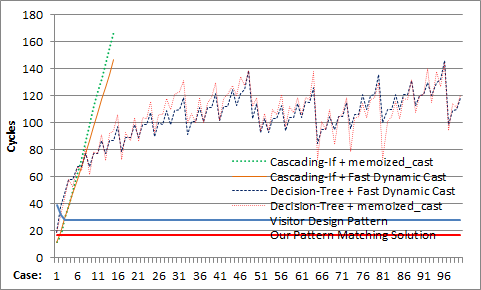
\includegraphics[width=0.47\textwidth]{DCast-vs-Visitors2.png}
  \caption{Type switch based on const-time type inclusion tests}
  \label{fig:DCastVis2}
\end{figure}

The chart in Figure~\ref{fig:DCastVis2} shows the time (Y-axis) each technique 
took to recognize an object of the most-derived type $i$ (X-axis). It is easy to 
see that the logarithmic cost associated with the decision tree very quickly 
surpasses the constant overhead of double dispatch present in the visitor design
pattern or the jump-table implementation of the switch on all tags. The edgy 
shape of timing results reflects the shape of the binary tree class hierarchy 
used for this experiment.
